\documentclass[journal, a4paper]{IEEEtran}
\usepackage{graphicx}   
\usepackage{url}
\usepackage{amsmath} 
\usepackage[utf8]{inputenc}
\usepackage{graphicx} 
\usepackage{float}
\usepackage{wrapfig}
\usepackage{pgfplots}
\usepackage{tikz}
\usepackage{cite}
\usetikzlibrary{positioning}
\DeclareMathAlphabet{\mathpzc}{OT1}{pzc}{m}{it}


\tikzset{%
   neuron missing/.style={
    draw=none, 
    scale=4,
    text height=0.333cm,
    execute at begin node=\color{black}$\vdots$
  },
}

\pgfplotsset{width = 5cm, compat=1.13}
\pgfplotsset{every axis/.append style={
    axis x line=middle,    % put the x axis in the middle
    axis y line=middle,    % put the y axis in the middle
    axis line style={<->}, % arrows on the axis
    },
    cmhplot/.style={color=blue,mark=none,line width=1pt,<->},
}

\begin{document}
	\title{Multimedia processing using machine learning}
	\author{Jakub Bielawa, Paweł Cejrowski, Łukasz Dawidowski, Łukasz Myśliński, Agata Radys}
	\markboth{Gdansk University of Technology, ETI department}{}
	\maketitle

\begin{abstract}
Some abstract
\end{abstract}

\section{Introduction}
The field of digital audio processing is an interesting topic, broadly investigated in scientific research. Problems such as music genre or instrument classification have been sucessfully solved in the past with the use of traditional machine learning methods. In this paper we analyse the results of "ISMIS 2011 Contest: Music Information Retrieval/Music Genres", and try to improve the results achieved in that challange. 
\section{Theory}
\subsection{Neural networks}
\subsubsection{Fully connected neural network}
A fully connected neural network (FCNN) is such a neural network in which each neuron is connected to every neuron in the previous layer and each connection has its own weight. \par This is a general purpose connection pattern and makes no assumptions about the features in the input data to recognize. This type of network is very expensive in terms of memory (weights) and computations (connections).
\begin{figure}[H]
\centering
\includegraphics[width=250px]{pictures/fcnn.png}
\caption{Fully connected neural network}
\end{figure}

\subsubsection{Convolutional neural network}
Convolutional neural network (CNN) is a type of feed-forward artificial neural network, which means that connections between the neurons do not form a cycle. Information in the network moves only forward so the given signal goes through the neuron once.
\par CNN includes a convolutional layer and usually few other hidden layers. Each neuron is connected only to a small region of the previous layer called receptive field. Receptive fields of different neurons are overlapping with other neuron's fields so that together they are covering the whole input.
\par CNN are used for image processing because while using convolution they can recognize edges of an object on the image.
\begin{figure}[H]
\centering
\includegraphics[width=250px]{pictures/cnn.png}
\caption{Convolutional neural network}
\end{figure}

\subsubsection{Recurrent neural network}
In recurrent neural network (RNN) connections between the neurons form a directed cycle. It means that RNN can use its internal memory to learn  sequences of inputs. The same set of weights is applied recursively to the structure.
\par RNN are used for text or speech recognition.
\begin{figure}[H]
\centering
\includegraphics[width=250px]{pictures/rnn.png}
\caption{Convolutional neural network}
\end{figure}

\subsection{Activation function}
The activation function defines the output of considered neuron with given input. There are many functions that can be used as an activation function in artificial neural networks. The most popular are:
\subsubsection{Linear}
\begin{center}
$ f(x)=ax + b $ \\ $ a,b \in R $ \\~\\
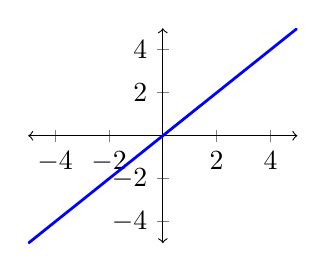
\begin{tikzpicture}
	\begin{axis}
		\addplot[cmhplot,-]{x};
	\end{axis}
\end{tikzpicture}
\end{center}

\subsubsection{Rectified Linear Unit (ReLU)}
\[
f(x)=
\left\{
\begin{array}{ll}
      0 ,& x < 0 \\
      x ,& x\geq 0 \\
\end{array} 
\right. \]
\begin{center}
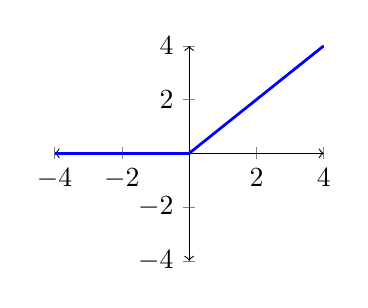
\begin{tikzpicture}
    \begin{axis}[
            xmin=-4,xmax=4,
            ymin=-4,ymax=4,
        ]
        \addplot[cmhplot,-,domain=-4:0]{0};
        \addplot[cmhplot,-,domain=0:4]{x};

    \end{axis}
\end{tikzpicture}
\end{center}

\subsubsection{Sigmoid}
\begin{center}
$f(x) = \frac{1}{1 + e^{-x}}$ \\
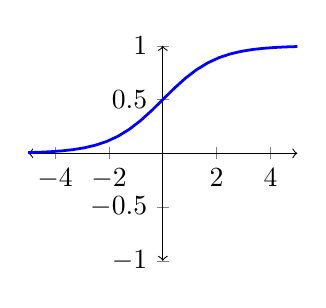
\begin{tikzpicture}
    \begin{axis}[
            xmin=-5,xmax=5,
            ymin=-1,ymax=1,
        ]
        \addplot[cmhplot,-]{1/(1 + e^(-x))};
    \end{axis}
\end{tikzpicture}
\end{center}

\subsubsection{TanH}
\begin{center}
$ f(x)=\tanh(x)=\frac{2}{1+e^{-2x}}-1 $ \\
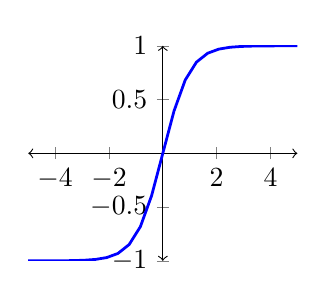
\begin{tikzpicture}
    \begin{axis}[
            xmin=-5,xmax=5,
            ymin=-1,ymax=1,
        ]
        \addplot[cmhplot,-]{2/(1 + e^(-2*x))-1};
    \end{axis}
\end{tikzpicture}
\end{center}

\subsection{Optimization and regularization}
\subsubsection{Dropout}
\subsubsection{Initial weights}
\subsubsection{Learning rate decay}
\subsubsection{Gradient Descent}

\subsection{Features}
An audio track in a digital format is represented by a discrete set of values identifying a sound wave. In order to apply machine learning techniques to a track, identifiers for each track is required. With the use of mathematical transformations like the Fourier transformation and its derivaties a collection of values representing each sample is aquired. In this particular study, the feature extraction process has already been applied. Features used are mainly based on MPEG-7 standard descriptors. Features represeting each track are listed below.

\begin{enumerate}
\item Temporal Centroid 
\item Spectral Centroid average value 
\item Audio Spectrum Envelope (ASE) average values in 31 frequency bands
\item ASE average value (averaged for all frequency bands)
\item ASE variance values in 31 frequency bands
\item averaged ASE variance parameters
\item Audio Spectrum Centroid – average and variance values
\item Audio Spectrum Spread – average and variance values
\item Spectral Flatness Measure (SFM) average values for 24 frequency bands
\item SFM average value (averaged for all frequency bands)
\item Spectral Flatness Measure (SFM) variance values for 24 frequency bands
\item Averaged SFM variance parameters
\item 20 first mel cepstral coefficients average values 
\item Harmonic Spectral centroid
\item Harmonic Spectral deviation
\item Harmonic Spectral spread
\item Harmonic Spectral variation
\item Harmonic Ratio average and variance values
\item Upper limit harmonicity average and variance values
\item Log attack time
\end{enumerate}

There parameters sum up to a total of 145 values used to identify track's musical identity. 


\section{Architecture}
As a solution for genre recognition problem, authors propose fully connected 4-hidden-layer neural network built up on TensorFlow framework. Hidden layers consist of $1024$, $1024$, $256$ and $56$ nodes. High-level architecture of the Depp Neural Network is presented in Figure \ref{fig:dnn}. Learning rate decaying is used with parameters as in equation \ref{eq:rate_decay}.
\begin{equation}
learning\ rate = 0.3 \times 0.9^{\frac{step}{500}}
\label{eq:rate_decay}
\end{equation}
Moreover, dropout is used during training after each of the hidden layers on the level of $0.7$, which means that $30\%$ is dropped out. After input layer and $4$ hidden layers ReLU activation function is used, whereas Softmax with cross entropy is used after the output layer. The network is optimized using Gradient Descent algorithm. Initial weights are randomly selected from $\mathcal{N}(0,0.05)$ for hidden layers and $\mathcal{N}(0,0.1)$ for output layer. Initial biases are set to $0$. 

\begin{figure}[H]%
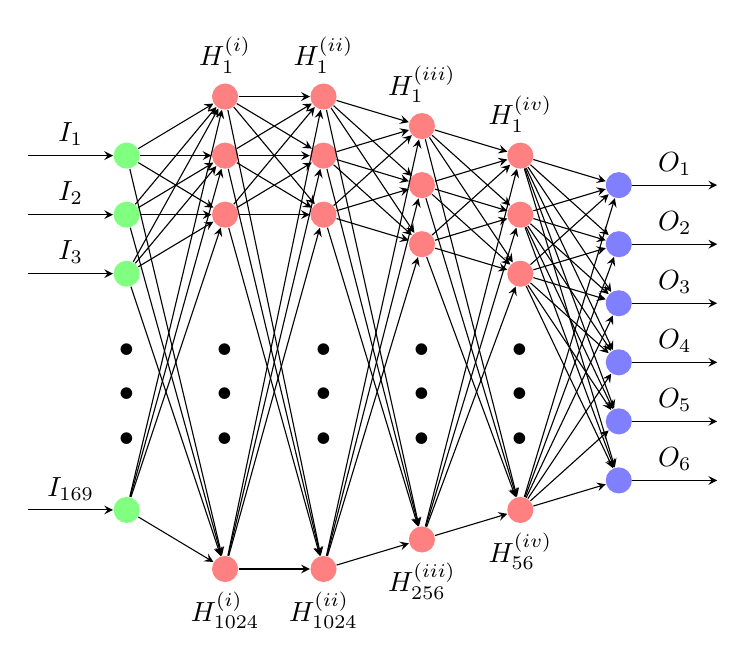
\begin{tikzpicture}[x=1.25cm, y=1.5cm, >=stealth]

\foreach \m/\l [count=\y] in {1,2,3}
{
 \node [circle,fill=green!50,minimum size=0.2cm] (input-\m) at (0,1.25-0.5*\y) {};
}
\foreach \m/\l [count=\y] in {4}
{
 \node [circle,fill=green!50,minimum size=0.2cm ] (input-\m) at (0,-1.25-\y) {};
}
 
 \node [neuron missing]  at (0,-1.25) {};
 

\foreach \m [count=\y] in {1,2,3}
  \node [circle,fill=red!50,minimum size=0.2cm ] (hidden1-\m) at (1,1.75-0.5*\y) {};
  
\foreach \m [count=\y] in {4}
  \node [circle,fill=red!50,minimum size=0.2cm ] (hidden1-\m) at (1,-2.75) {};
  
 \node [neuron missing]  at (1,-1.25) {};



\foreach \m [count=\y] in {1,2,3}
  \node [circle,fill=red!50,minimum size=0.2cm ] (hidden2-\m) at (2,1.75-0.5*\y) {};
  
\foreach \m [count=\y] in {4}
  \node [circle,fill=red!50,minimum size=0.2cm ] (hidden2-\m) at (2,-2.75) {};
  
 \node [neuron missing]  at (2,-1.25) {};



\foreach \m [count=\y] in {1,2,3}
  \node [circle,fill=red!50,minimum size=0.2cm ] (hidden3-\m) at (3,1.5-0.5*\y) {};
  
\foreach \m [count=\y] in {4}
  \node [circle,fill=red!50,minimum size=0.2cm ] (hidden3-\m) at (3,-2.5) {};
  
 \node [neuron missing]  at (3,-1.25) {};



\foreach \m [count=\y] in {1,2,3}
  \node [circle,fill=red!50,minimum size=0.2cm ] (hidden4-\m) at (4,1.25-0.5*\y) {};
  
\foreach \m [count=\y] in {4}
  \node [circle,fill=red!50,minimum size=0.2cm ] (hidden4-\m) at (4,-2.25) {};
  
 \node [neuron missing]  at (4,-1.25) {};



% output layer
\foreach \m [count=\y] in {1}
  \node [circle,fill=blue!50,minimum size=0.2cm ] (output-\m) at (5,1.5-\y) {};
\foreach \m [count=\y] in {2}
  \node [circle,fill=blue!50,minimum size=0.2cm ] (output-\m) at (5,1.0-\y) {};
\foreach \m [count=\y] in {3}
  \node [circle,fill=blue!50,minimum size=0.2cm ] (output-\m) at (5,0.5-\y) {};
\foreach \m [count=\y] in {4}
  \node [circle,fill=blue!50,minimum size=0.2cm ] (output-\m) at (5,0.0-\y) {};
\foreach \m [count=\y] in {5}
  \node [circle,fill=blue!50,minimum size=0.2cm ] (output-\m) at (5,-0.5-\y) {};
\foreach \m [count=\y] in {6}
  \node [circle,fill=blue!50,minimum size=0.2cm ] (output-\m) at (5,-1.0-\y) {};

%%%%%%%%%%%%%%%%%%%%%%%%%%%%%%%%%%%%%%%%%%%%%%%%%%%%%%%%%%%%%%%%%%%%%%%%%%%%%
% labels

\foreach \l [count=\i] in {1,2,3,169}
  \draw [<-] (input-\i) -- ++(-1,0)
    node [above, midway] {$I_{\l}$};

\foreach \l [count=\i] in {1}
  \node [above] at (hidden1-\i.north) {$H^{(i)}_{\l}$};

\foreach \l [count=\i] in {1}
  \node [above] at (hidden2-\i.north) {$H^{(ii)}_{\l}$};

\foreach \l [count=\i] in {1}
  \node [above] at (hidden3-\i.north) {$H^{(iii)}_{\l}$};

\foreach \l [count=\i] in {1}
  \node [above] at (hidden4-\i.north) {$H^{(iv)}_{\l}$};

\foreach \l [count=\i] in {1024}
  \node [below] at (hidden1-4.south) {$H^{(i)}_{\l}$};

\foreach \l [count=\i] in {1024}
  \node [below] at (hidden2-4.south) {$H^{(ii)}_{\l}$};

\foreach \l [count=\i] in {256}
  \node [below] at (hidden3-4.south) {$H^{(iii)}_{\l}$};

\foreach \l [count=\i] in {56}
  \node [below] at (hidden4-4.south) {$H^{(iv)}_{\l}$};



\foreach \l [count=\i] in {1,2,3,4,5,6}
  \draw [->] (output-\i) -- ++(1,0)
    node [above, midway] {$O_{ \l}$};
		
%%%%%%%%%%%%%%%%%%%%%%%%%%%%%%%%%%%%%%%%%%%%%%%%%%%%%%%%%%%%%%%%%%%%%%%%%%%%%
% connections

\foreach \i in {1,...,4}
  \foreach \j in {1,...,4}
    \draw [->] (input-\i) -- (hidden1-\j);

\foreach \i in {1,...,4}
  \foreach \j in {1,...,4}
    \draw [->] (hidden1-\i) -- (hidden2-\j);
\foreach \i in {1,...,4}
  \foreach \j in {1,...,4}
    \draw [->] (hidden2-\i) -- (hidden3-\j);
		\foreach \i in {1,...,4}
  \foreach \j in {1,...,4}
    \draw [->] (hidden3-\i) -- (hidden4-\j);
\foreach \i in {1,...,4}
  \foreach \j in {1,...,6}
    \draw [->] (hidden4-\i) -- (output-\j);

\end{tikzpicture}
\caption{Deep neural network schema}%
\label{fig:dnn}%
\end{figure}


	
\section{Experiments}
For experiments data from \cite{data} was used. Only Training dataset had labels, so it was randomly split in half, so that both the training and test datasets contained of $6248$ observations. Duplicate columns were dropped before feeding the neural network. After using different configuration settings training procedure was established on $3001$ steps with batches of size $128$ observations.  We have made experiments, tuning our neural network parameters and get $96.4\%$ accuracy on test data.

\section{Further Research}
In the presented research authors investigated complete end to end solution for classic genre recognition problem. It is possible to improve the proposed approach in a the following fields:
\begin{itemize}
 \item more features can be extracted from audio files,
 \item RNN can be applied to features so that correlations between consecutive frames are better highlighted,
 \item frame overlapping can be applied,
 \item more regularization is needed to decrease batch overfitting.
\end{itemize}
Mentioned areas are going to be the subject of further investigation on the subject.


\section{Conclusions}

Results are partially satisfying. While a very good result on an established dataset from \cite{data} was obtained, an attempt to process raw sound database, such as in \cite{gztan} has failed to deliver good results. In order to decisively establish the legitimacy of the networks architecture further research is required. Validating against more datasets is desirable.

\bibliography{bibliography}{}
\bibliographystyle{plain}
\end{document}
